\subsection{Etap Plan}
Faza planowania (\textit{Plan}) odpowiada za zdefiniowanie wymagań, priorytetyzację zadań i organizację pracy. W niniejszym projekcie etap ten realizowany jest z użyciem platformy Jira jako centrum zarządzania backlogiem.

\subsubsection{Zarządzanie projektami: Jira}
Do zarządzania wymaganiami i planowania prac wykorzystano platformę \textbf{Jira} (projekt \textit{INZ}). Narzędzie to wybrano, ponieważ jest standardem rynkowym i oferuje zaawansowane możliwości obsługi metodyk zwinnych (Agile).

\textbf{Metodyka:}
Agile to rodzina iteracyjnych metodyk wytwarzania oprogramowania, kładących nacisk na częste dostarczanie wartości i adaptację do zmian. Sprinty są podstawową jednostką iteracji w Agile — to ograniczone czasowo okresy pracy (zazwyczaj 1--4 tygodnie), po których dostarcza się działający przyrost produktu. Tablica Kanban to uproszczona alternatywa skupiona na wizualizacji przepływu zadań i ograniczaniu pracy w toku, bez sztywnych iteracji czasowych.

Ponieważ projekt realizowany jest indywidualnie i w ograniczonym czasie, zadania podzielono logicznie na sprinty zgodnie z etapami pętli DevOps, lecz do bieżącego śledzenia pracy zastosowano tablicę Kanban — bardziej odpowiednią dla małych, jednoosobowych projektów.

\textbf{Struktura backlogu:}
Backlog projektu odwzorowuje etapy pętli DevOps. Zdefiniowano pięć Epics odpowiadających sprintom implementacyjnym: \textit{Build}, \textit{Release}, \textit{Deploy}, \textit{Monitor} i \textit{Polish}. W ramach każdego Epica utworzono zestaw zadań (\textit{Tasks}) pokrywających zarówno dostarczenie kodu infrastruktury, jak i uzupełnienie odpowiednich sekcji pracy inżynierskiej. Łącznie backlog liczy 29 zadań.

\textbf{Integracja i dobre praktyki:}
Zastosowano integrację z systemem kontroli wersji GitHub. Każda gałąź kodu (\textit{branch}) jest nazwana według schematu \texttt{feature/INZ-XX-opis}, a wiadomości zatwierdzeń zawierają identyfikator zadania (np. \texttt{feat(helm): INZ-9 create umbrella chart}). Dzięki temu zmiany w kodzie są automatycznie powiązane z odpowiednim zgłoszeniem w Jira, co zapewnia pełną identyfikowalność — od wymagania po konkretną linię kodu.

\begin{figure}[H]
    \centering
    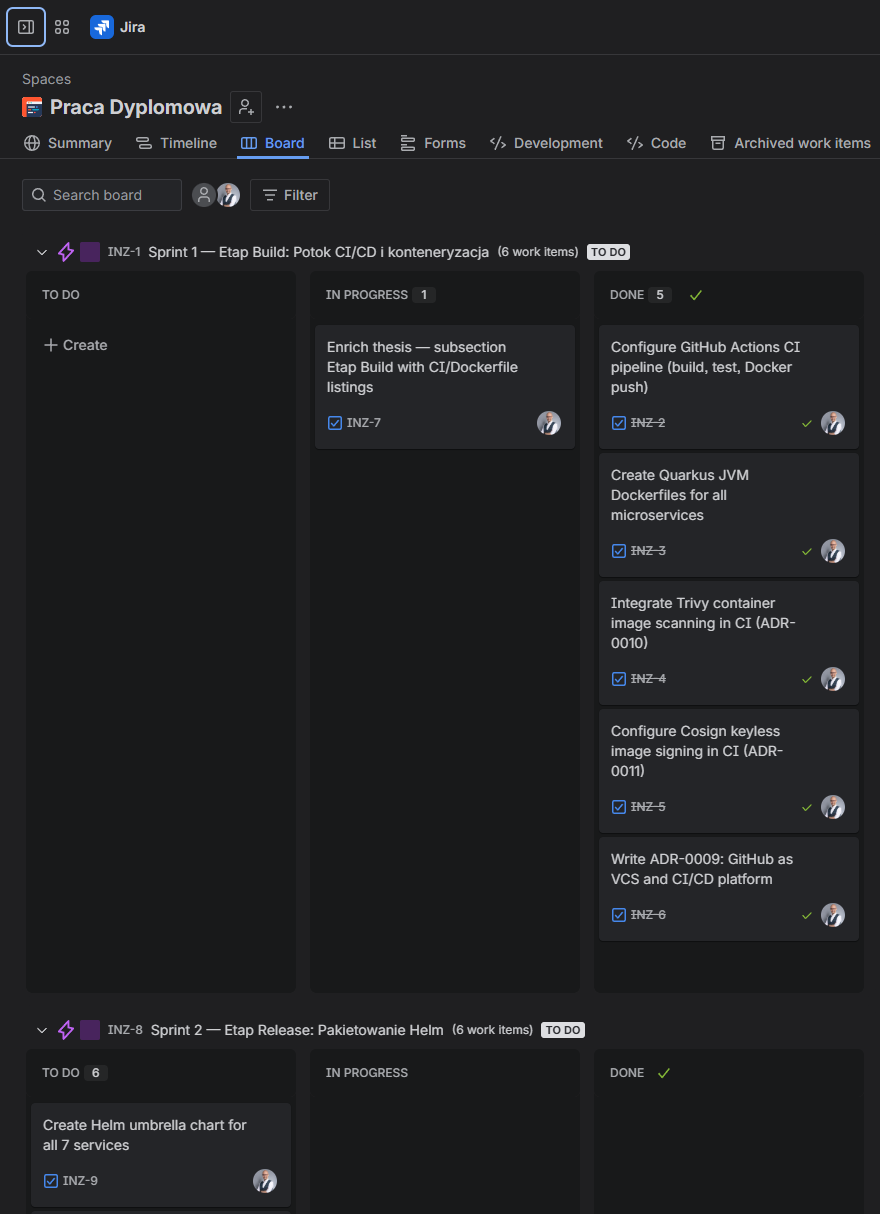
\includegraphics[width=0.75\textwidth]{jira.png}
    \caption{Tablica Kanban projektu INZ w Jira -- widok sprintów i zadań}
    \label{fig:jira-board}
\end{figure}
